
\section{Tema 1: Introducción y generalidades sobre metrología}
\subsection{Definiciones}
\begin{enumerate}
	\item \underline{\textbf{Magnitud}}: Atributo de un cuerpo que se puede distinguir cualitativamente y determinado cuantitativamente.
	\item \underline{\textbf{Magnitud básica}}: Magnitud que se acepta como independiente.
	\item \underline{\textbf{Magnitud derivada}}: Se define en a través de las magnitudes básicas.
	\item \underline{\textbf{Unidad de medida}}: Magnitud adoptada por convenio con la que se comparan magnitudes de la misma naturaleza.
	\item \underline{\textbf{Unidad coherente}}: Unidad derivada expresada como producto de potencias de unidades básicas.
	\item \underline{\textbf{Sistema de unidades}}: Conjunto de unidades básicas y derivadas. Cabe destacar el Sistema Internacional de Unidades que es un sistema coherente de unidades adaptado por la Conferencia General de Pesas y Medidas.
	\item \underline{\textbf{Valor de una magnitud}}: Expresión cuantitativa de una magnitud. Se expresa como una unidad de medida multiplicada por un número.
	\item \underline{\textbf{Valor verdadero}}: Valor que se obtendría a través de una medición perfecta de una magnitud. Este valor nunca se puede determinar, todas las medidas introducen incertidumbre.
	\item \underline{\textbf{Valor convencionalmente verdadero}}: Valor más probable que toma una magnitud. Se debe acompañar con su incertidumbre. Normalmente se corresponde con la media.
	\item \underline{\textbf{Medida}}: Conjunto de operaciones para determinar el valor de una magnitud. 
	\item \underline{\textbf{Medición general}}: Se determina el valor de una magnitud sobre la que se realiza alguna acción de control. Se realiza mediante aparatos convencionales.
	\item \underline{\textbf{Medición metrológica}}: Procedimiento plenamente especificado con el fin de calibrar o verificar un aparato. Se requieren aparatos patrones.
	\item \underline{\textbf{Mensurando}}: Magnitud sometida a medición.
	\item \underline{\textbf{Magnitud de influencia}}: Magnitudes que no son el objetivo de la medida pero alteran la medición.
	\item \underline{\textbf{Señal de medida}}: Magnitud que mantiene una relación funcional con el mensurando y lo representa.
	\item \underline{\textbf{Cadena de medida}}: Conjunto de instrumentos y personas que intervienen en una medición.
	\item \underline{\textbf{Valor nominal}}: Valor aproximado de una característica de un instrumento. 
	\item \underline{\textbf{Campo de medida (CM)}}: Valor máximo que puede indicar un aparato.
	\item \underline{\textbf{Rango de medida}}: Intervalo en el que el error debido al instrumento de medida se mantiene en unos límites especificados.
	\item \underline{\textbf{Constante de medida}}: Número por el que debe multiplicarse la medida de un instrumento para obtener el valor del mensurando. 
	\begin{center} 	Normalmente en un aparato analógico:\end{center}
		\[ k_m = \frac{CM}{Divisiones} \]
	\item \underline{\textbf{Estabilidad}}: Aptitud de un instrumento para mantener constantes sus características a lo largo del tiempo.
	\item \underline{\textbf{Transparencia}}: Aptitud de un instrumento para no alterar el mensurando.
	\item \underline{\textbf{Deriva}}: Variación lenta de una característica del instrumento por el paso del tiempo, mal uso o desgaste.
	\item \underline{\textbf{Zona muerta}}: Máxima variación de la señal de entrada sin que se perciba respuesta en la salida.
	\item \underline{\textbf{Sensibilidad}}: Variación de la salida ante un incremento de la entrada. No tienen porque ser siempre iguales.
	\[ S(x) = \frac{dx}{dy}=\frac{\bigtriangleup x}{\bigtriangleup y} \]
	\item \underline{\textbf{Resolución}}: Menor diferencia que puede apreciarse en un aparato de manera significativa.
	\begin{itemize}
	 \item En un aparato analógico suele tomarse como E/2 y como máximo E/4 donde E es una división de escala.
	 \item En un aparato digital se suele tomar su dígito menos significativo.
	\end{itemize}
	
	\begin{figure}[H]
		\centering
		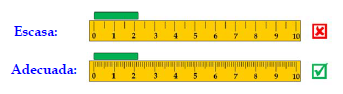
\includegraphics[width=0.5\textwidth]{imagenesTema1/resolucion.png}  
		\caption{Comparativa de resoluciones}
		\label{fig:sample}
	\end{figure}
	
	
	\item \underline{\textbf{Veracidad}}: Concordancia entre la media de un conjunto de medidas y un valor de referencia. Normalmente se comprueba si un valor nominal es correcto.
	\item \underline{\textbf{Precisión}}: Capacidad de un instrumento para dar valores agrupados al repetir medidas.
	\item \underline{\textbf{Exactitud}}: Grado de concordancia entre un valor medido y el verdadero. Requiere veracidad y precisión.
	\item \underline{\textbf{Sesgo}}: Diferencia entre la media de las medidas y el valor de referencia.
	\item \underline{\textbf{Linealidad}}: Indica la evolución del sesgo a lo largo del campo de medida del aparato.
	
	\begin{figure}[H]
		\centering
		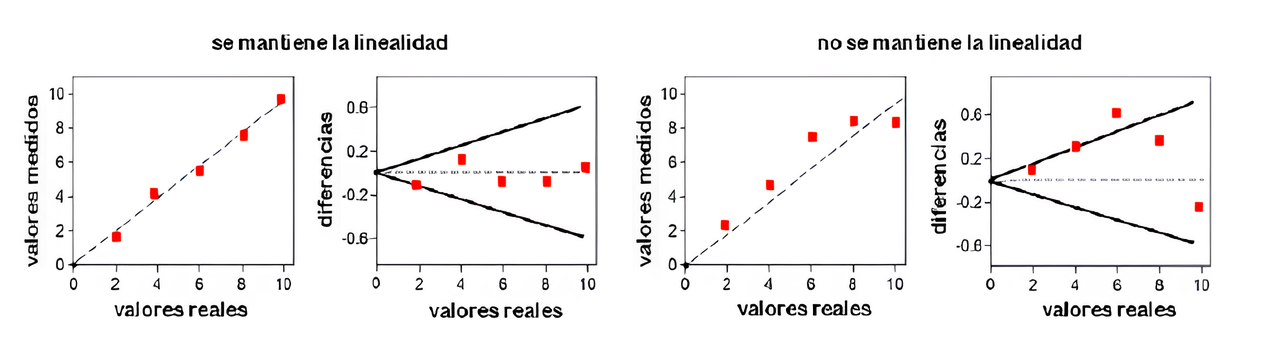
\includegraphics[width=1\textwidth]{imagenesTema1/linealidad.png}  
		\caption{Comparativa de resoluciones}
		\label{fig:sample}
	\end{figure}
	
	\item \underline{\textbf{Índice de clase}}: Número que informa sobre la exactitud de un aparato según su calidad metrológica. El índice se define como: 
	\[C_A = \frac{100 \alpha}{CM} \rightarrow \alpha = \text{ Error absoluto máximo}\]	

	Como el índice solo da información del error absoluto, el punto donde se calcula es aquel en el que el error relativo es mínimo. Viéndolo gráficamente:

	\begin{figure}[H]
		\centering
		\begin{tikzpicture}[scale=0.7]
			\begin{axis}[
				xlabel=$Lectura$,
				ylabel=$Error relativo (\%)$,
				xmin=0, xmax=10,
				ymin=0, ymax=5,
				axis lines=center,
				 xlabel style={at={(current axis.right of origin)}, anchor=west, yshift=-20pt},
				ylabel style={at={(current axis.above origin)}, anchor=south, xshift=-10pt, rotate=90 }
				]
				\addplot[domain=0.01:10, samples=100, blue] {1/x};
			\end{axis}
			
		\end{tikzpicture}
		\caption{Gráfica del error del aparato a lo largo del campo de medida}
		\label{fig:graph-1-over-x}
	\end{figure}

	Este índice sirve para evaluar la incertidumbre intrínseca de un instrumento de medida.
	\renewcommand{\arraystretch}{1.1} % Adjust the factor as needed
	\begin{table}[htb]
		\centering
		\begin{tabular}{|c|c|c|c|}
			\hline
			{} &\textbf{Laboratorio} & \textbf{Uso industrial} & \textbf{Indicadores} \\
			
			\hline
			$C_A$ & 0.05 - 0.1 - 0.2 - 0.5 & 1 - 1.5 - 2.5 & 5 \\
			\hline
		\end{tabular}
		\caption{Tabla de clases de aparatos}
		\label{tab:your-table-label}
	\end{table}
	
	En aparatos digitales la clase también suele incluir un termino proporcional a la lectura del aparato:
	\[C_D= X\% CM + Y\% L \]
	
	\item \underline{\textbf{Incertidumbre de medida}}: Parámetro asociado al resultado de una medición. Caracteriza la dispersión de los valores. Se expresa acompañando a la medida mediante la incertidumbre expandida (normalmente k=2).
	
	\[U(x) = k u(X) \]
	\begin{itemize}
		\item U(x) $\rightarrow$ Incertidumbre expandida
		\item k $\rightarrow$ Factor de cobertura. Mide el nivel de confianza sobre el mensurando.
		
		\renewcommand{\arraystretch}{1.1} % Adjust the factor as needed
		\begin{table}[htb]
			\centering
			\begin{tabular}{|c|c|c|c|c|c|}
				\hline
				{k} &\textbf{1} & \textbf{2} & \textbf{3}  & \textbf{4}& \textbf{5} \\
				
				\hline
				Porcentaje datos&68.27\% & 95.45\% & 99.73\% & 99.994\% & 99.99994\% \\
				
				\hline
			\end{tabular}
			\caption{Tabla de intervalos cobretura}
			\label{tab:your-table-label}
		\end{table}
		
		\item u(X) $\rightarrow$ Incertidumbre sin expandir.
	\end{itemize} 
	
	Normalmente la incertidumbre es el resultado de combinar diferentes componentes y se emplea para comparar la calidad de las medidas.
	\item \underline{\textbf{Error de medida }}: Diferencia entre el resultado de una	medición y el valor real del mensurando.
	\item \underline{\textbf{Error aleatorio}}:Diferencia entre el resultado de una medición y la media de infinitas medidas en condiciones de repetibilidad.
	\\
	Para minimizar este error se deben emplear múltiples medidas y utilizar la media aritmética como estimador de la medición.
	\item \underline{\textbf{Error sistemático}}: Diferencia entre la media de infinitas medidas realizadas en condiciones de repetibilidad y el valor verdadero del mensurando.
	\\
	Si se conoce la causa del error puede eliminarse aplicando correcciones.
	
	\begin{figure} [H]
		\centering
		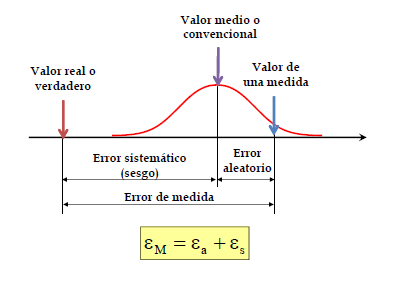
\includegraphics[width=1\textwidth]{imagenesTema1/errormedida.png}  
		\caption{Errores representados gráficamente}
		\label{fig:sample}
	\end{figure}
	\item \underline{\textbf{Tolerancia}}: Intervalo de valores dentro del cual debe situarse el valor real de una magnitud para que se acepte como válida. Es un indicador de un elemento.
	Si el limite inferior $LSE$ y superior $LIE$ se encuentran equidistantes al valor nominal.
	
	\[T=\pm \frac{LSE - LIE}{2}\]

\end{enumerate}

\subsection{Ley propagación de incertidumbres}
\begin{enumerate}
	\item \underline{Medidas independientes}: Las variables $x_i$ son independientes entre sí:
	\[y=f(x_1,x_2,\ ... \ ,x_n)\]
	\[u^2_y=  \left({\frac{\partial y}{\partial x_1}u_1}\right)^2 +
	\left({\frac{\partial y}{\partial x_2} u_2}\right)^2 + ... +
	\left({\frac{\partial y}{\partial x_i}u_i}\right)^2\]
	Tras hallar la incertidumbre a través de las incertidumbres sin expandir se expande mediante k.
	\item \underline{Medidas correlacionadas}: Cuando algunas variables están ligadas entre sí:
	\[y=f(x_1,x_2,\ ... \ ,x_n)\]
	\[u^2_y=   \sum_{i=1}^{n} \left({\frac{\partial y}{\partial x_i}u_i}\right)^2 + 2 \sum_{i=1}^{n} \sum_{j>i}^{n} \frac{\partial y}{\partial x_i} \frac{\partial y}{\partial x_j} r_{ij} u_i u_j
	\]
	Donde $r_{ij}$ son los coeficientes de correlación entre las variables.
	\item \underline{Mediante errores porcentuales}:
		\begin{itemize}
			\item Producto de variables:
			\[y= x_1 x_2\]
			\begin{itemize}		
				\item Sin correlación:
				\[u_y^2=  ({x_2 u_1})^2 +({x_1 u_2})^2\]
				Dividiendo por: $(x_1 x_2)^2$
				\[u_{y(pu)}^2=   u_{1(pu)}^2 +u_{2(pu)}^2\]
				\item Con correlación:
				\[u_{y(pu)}^2=   u_{1(pu)}^2 +u_{2(pu)}^2+2ru_{1(pu)}u_{2(pu)}\]
			\end{itemize}
			\item Cociente de variables:
			\[y= \frac{x_1} {x_2}\]
			\begin{itemize}
				\item Sin correlación:
				\[u_y^2=  \left({\frac{ u_1}{x_2}}\right)^2 +\left({\frac {x_1 u_2}{x_2^2}}\right)^2\]
				Dividiendo por: $\left({\frac{ x_1}{x_2}}\right)^2$
				\[u_{y(pu)}^2=   u_{1(pu)}^2 +u_{2(pu)}^2\]
				\item Con correlación:
				\[u_{y(pu)}^2=   u_{1(pu)}^2 +u_{2(pu)}^2-2ru_{1(pu)}u_{2(pu)}\]
			\end{itemize}
			\item Potencia de una variable:
			\[y= x^n\]
			\begin{itemize}
				\item Sin correlación:
					\[u_y=n x^{n-1}u_x\]
				Dividiendo por: $ x^{n}$
				\[u_{y(pu)}=  n u_{1(pu)}\]

			\end{itemize}
		\end{itemize}
		Este método, se emplea para evitar el cálculo de derivadas parciales y se aplican combinados.
\end{enumerate}
\subsection{Estimación de la incertidumbre}
\begin{enumerate}
	\item \underline{Incertidumbres de tipo A}: Se basan en datos de resultados experimentales. Se obtiene la media y la incertidumbre a partir de las medidas.
	\\La incertidumbre es la desviación típica de la media:
	\[ \bar x = \sum_{i=1}^{n} \frac{x_i}{n} \]
	\[\hat{s}=\sqrt[]{\sum_{n=1}^n \frac{(x_i -x)^2}{n-1}} \]
	\begin{itemize}
		\item Medidas independientes:
		\[ u_A^2(\bar x) =  \frac{\hat{s}^2}{n} \rightarrow u_A(\bar x) =  \frac{\hat{s}}{\sqrt[]{n}}\]
		\item Medidas dependientes:
		\[ u_A^2(\bar x) =  \frac{\hat{s}^2}{n} + r \left({\frac{n-1}{n}}\right)\hat{s}^2\]
	\end{itemize}
	\item \underline{Incertidumbres de tipo B}: Se basan en datos de mediciones anteriores. Se suele estimar en base al alcance de la medida y al tipo de distribución. Requieren el conocimiento del aparato de medida.
	\begin{flushleft}
	El valor de $\alpha$ se corresponde con el error absoluto máximo de la clase del aparato. Normalmente si no se dice nada la distribución se asume rectangular.
\end{flushleft}
		\begin{figure}[H]
		\centering
		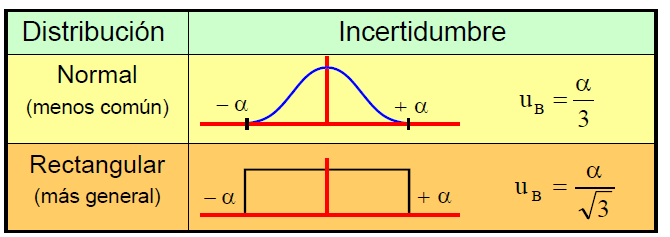
\includegraphics[width=0.5\textwidth]{imagenesTema1/tipob.png}  
		\caption{Incertidumbre según la distribución}
		\label{fig:sample}
	\end{figure}
	
\end{enumerate}
\newpage
\subsection{Relación tolerancia incertidumbre}
Las tolerancias son la base del principio de intercambiabilidad. Para ello, es necesario medir y así saber si una magnitud está en tolerancia. No obstante, si la incertidumbre es incorrecta puede dar lugar a fallos ocultos o falsos fallos.
 \begin{figure} [H]
 	\centering
 	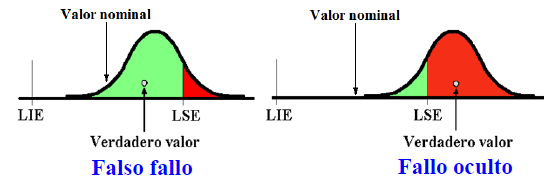
\includegraphics[width=1\textwidth]{imagenesTema1/tolerancia.png}  
 	\caption{Problemas relación tolerancia incertidumbre}
 	\label{fig:sample}
 	\end{figure}
 	
En la práctica se opta por rechazar cualquier mensurando que este fuera de la tolerancia efectiva:
 \[T_{eff}=T-2U\]
 Si T está centrada, suele considerarse admisible mantener:
 \[3\leq \frac{T}{U} \leq 10\]
 S T no está centrada, entonces:
  \[3\leq \frac{T}{2U} \leq 10\]
 
 \begin{figure} [H]
 	\centering
 	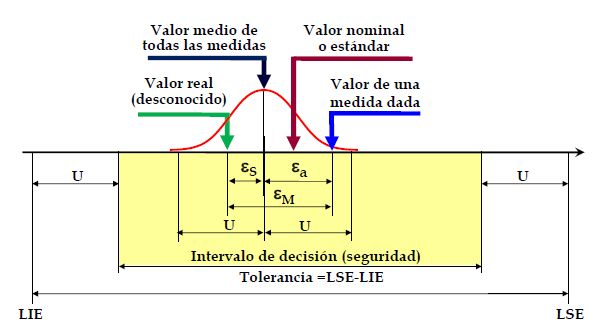
\includegraphics[width=0.8\textwidth]{imagenesTema1/resumen.png}  
 	\caption{Problemas relación tolerancia incertidumbre}
 	\label{fig:sample}
 \end{figure}
 	
\subsection{Resumen magnitudes estudiadas en el bloque}
Si existe demasiada resolución las lecturas pueden tener más cifras significativas de las necesaria. No obstante, con poca resolución las variación no serán apreciables.
\begin{enumerate}
	\item Aparatos analógicos
	\[0.5\leq \frac{U(k \geq 2)}{E} \leq 10\]
	\item Aparatos digitales
		\[0.5\leq \frac{U}{E} = \frac{\alpha}{dms}\]
		Donde $dms$ es el dígito menos significativo.
\end{enumerate}
\subsection{Reglas redondeo}
\begin{enumerate}
	\item Si la última cifra es menor a 5 se redondea por defecto.

	\item Si la última cifra es mayor a 5 se redondea por exceso.
	
	
	\item Si la última cifra es 5.
	\begin{enumerate}
			\item Si la cifra anterior es par se redondea por defecto.
			\item Si la cifra anterior es impar se redondea por exceso.
	\end{enumerate}
\end{enumerate}
